% Provenance (never printed): old terminale S material on the continental crust
% (granitic composition, thickness, density, age; roots and isostasy). Thickness
% from Christensen-Mooney 1995 and Cogley 1984 (CRUST1.0 dropped: no licence,
% Sync 1); ocean-floor ages from figdata/grade-12/crust_ages.py (Seton 2020 grid,
% as in g11.01). Airy isostasy is g11.03's: recalled, not re-derived. Radiometric
% dating is g12.07's: ages are only quoted here.
\chapter{La corteza continental}\label{ch:g12:continental-crust}

En el noroeste de Canadá, cerca del río Acasta, aflora una roca gris
surcada de bandas claras y oscuras. Se ha datado en 4000 a 4030 millones de
años: es el gneis de Acasta, la roca más antigua que se conoce. Más antiguos
aún son unos granos del mineral circón, cada uno de una fracción de milímetro,
hallados en viejas rocas sedimentarias de las Jack Hills, en Australia
Occidental. Arrancados de rocas más antiguas y transportados por el agua antes
de quedar enterrados, cristalizaron hace 4400 millones de años, y muestran que
ya existía entonces una corteza. Ningún fondo oceánico tiene ni la vigésima
parte de esa edad. Este capítulo se pregunta de qué están hechos los
continentes y por qué perduran.
% ledger: bowring99:acasta, wilde01:zircon, uw14:jack-hills, photo:g12-acasta, photo:g12-jack-hills-zircons

\begin{omfigure}
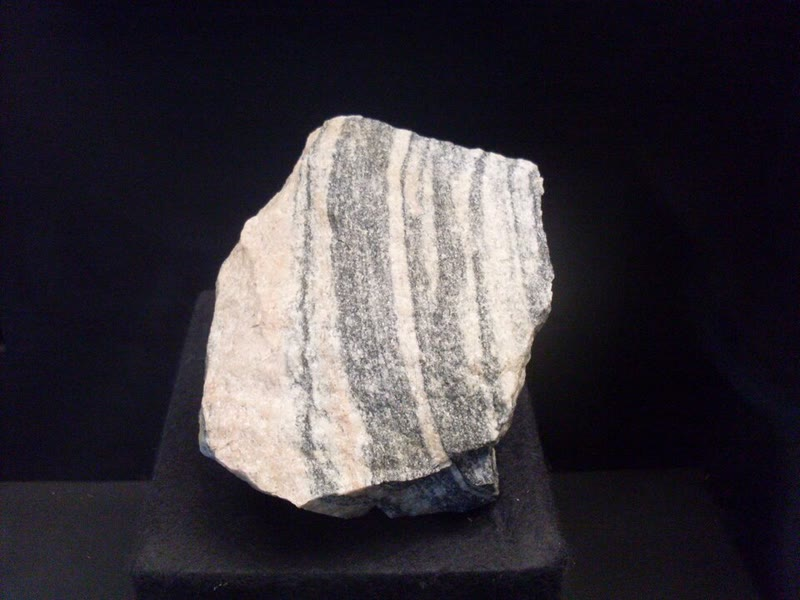
\includegraphics[height=4.6cm]{images/book2/g12-pedro-acasta-gneiss.jpg}\hspace{0.04\linewidth}%
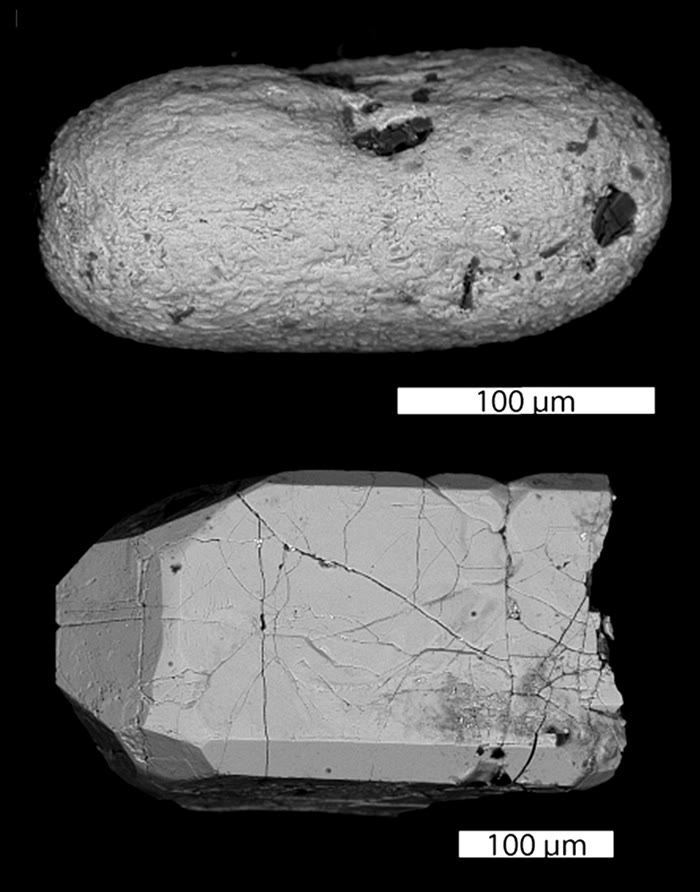
\includegraphics[height=4.6cm]{images/book2/g12-cavosie-jack-hills-zircons.jpg}

{\small A la izquierda: un fragmento del gneis de Acasta, de 4030 millones de
años, expuesto en un museo. Fotografía de Pedroalexandrade (CC~BY-SA~3.0). A
la derecha: dos granos de circón de las Jack Hills, Australia Occidental,
vistos con un microscopio electrónico; cada barra de escala mide
\qty{100}{\micro m}. El grano de arriba se redondeó al ser transportado por el
agua; el de abajo conservó sus caras cristalinas. Imágenes de A.~Cavosie y
J.~Valley (dominio público).}
\end{omfigure}
% ledger: photo:g12-acasta, photo:g12-jack-hills-zircons

\begin{recall}
La corteza termina en el \omterm{def:g11:seismic-structure:moho}{Moho}, bajo el cual se encuentra el manto, más denso
(el \cref{ch:g11:seismic-structure}). La \omterm{def:g11:ocean-ridges:oceanic-lithosphere}{corteza oceánica} consta de unos
\qty{7}{km} de basalto y \omterm{def:g11:ocean-ridges:gabbro}{gabro} formados en las dorsales (el
\cref{ch:g11:ocean-ridges}), y nunca tiene más de unos 190 millones de años
(el \cref{ch:g11:drift-to-spreading}). Las capas externas flotan sobre la
\omterm{def:g11:lithosphere-asthenosphere:lithosphere}{astenosfera}: en el modelo de Airy, una región que se eleva una altura $h$ más
tiene una corteza más gruesa en $h\,\rho_m/(\rho_m -
\rho_c)$ (el \cref{ch:g11:lithosphere-asthenosphere}). Las rocas ígneas se
nombran por su \omterm{def:g11:igneous-rocks:texture}{textura} y su contenido en sílice: \omterm{def:g11:igneous-rocks:felsic-mafic}{máficas} de 45 a
\qty{55}{\percent} de \ce{SiO2}, \omterm{def:g11:igneous-rocks:felsic-mafic}{intermedias} de 55 a 65, \omterm{def:g11:igneous-rocks:felsic-mafic}{félsicas} de 65 a
75 (el \cref{ch:g11:igneous-rocks}). Los elementos radiactivos se desintegran
a un ritmo constante, lo que da su edad a las rocas (los libros de física;
el \cref{ch:g12:age-of-the-earth}).
\end{recall}
% ledger: white92:crust, data:b2-seafloor-age, tulane:magma-types

\section{De qué están hechos los continentes}

\begin{definition}[Corteza continental]\label{def:g12:continental-crust:continental-crust}
La \emph{corteza continental}\index{corteza continental} es la corteza que
forma los continentes, incluidas sus partes cubiertas por mares poco
profundos. Es gruesa, de composición granítica por término medio en su parte
superior, ligera, y puede ser muy antigua.
\end{definition}
% ledger: tulane:crust-types, tulane:roots, cogley84:continents

Los continentes son más grandes que las tierras emergidas. Los bordes de la
\omterm{def:g12:continental-crust:continental-crust}{corteza continental} están bajo el mar, en las plataformas continentales:
cartografiada así, la \omterm{def:g12:continental-crust:continental-crust}{corteza continental} cubre \num{210}~millones de~\unit{km^2},
el \qty{41}{\percent} de la superficie terrestre, del que casi un tercio, el
\qty{30.6}{\percent}, está sumergido. Contando sus partes sumergidas, la altura
media de la \omterm{def:g12:continental-crust:continental-crust}{corteza continental} es de solo unos \qty{120}{m} sobre el nivel
del mar.
% ledger: cogley84:continents

En la superficie, los continentes muestran todo tipo de rocas ---sedimentos,
\omterm{def:g11:igneous-rocks:volcanic-plutonic}{rocas volcánicas}, rocas metamórficas---, pero bajo la cobertera sedimentaria
la \omterm{def:g12:continental-crust:continental-crust}{corteza continental} está formada sobre todo por rocas graníticas y por las
rocas metamórficas y \omterm{def:g11:igneous-rocks:volcanic-plutonic}{plutónicas} de antiguas raíces de montañas. Por término
medio, la \omterm{def:g12:continental-crust:continental-crust}{corteza continental} entera contiene un \qty{60.6}{\percent} de
sílice; su parte superior es más rica, un \qty{66.6}{\percent}, así que su
parte profunda debe de ser más pobre.
% ledger: rg14:crust, tulane:crust-types, cm95:crust

\begin{omfigure}
\begin{tikzpicture}
\begin{axis}[omrecord, ybar=0pt, width=0.92\linewidth, height=5.0cm, bar width=7pt,
  ymin=0, ymax=80, ylabel={fracción en masa (\unit{\percent})},
  symbolic x coords={SiO2, Al2O3, FeO, MgO, CaO, Na2O, K2O},
  xticklabels={\ce{SiO2}, \ce{Al2O3}, \ce{FeO}, \ce{MgO}, \ce{CaO}, \ce{Na2O}, \ce{K2O}},
  xtick=data, enlarge x limits=0.08, ymajorgrids=true, xmajorgrids=false,
  legend style={font=\scriptsize, at={(0.98,0.97)}, anchor=north east, legend columns=1}]
% ledger: rg14:crust (upper and bulk continental crust; FeO* total iron)
\addplot[fill=omLithGranite, draw=black!60] coordinates {(SiO2,66.6) (Al2O3,15.4) (FeO,5.04) (MgO,2.48) (CaO,3.59) (Na2O,3.27) (K2O,2.80)};
\addplot[fill=omProp!55, draw=black!60] coordinates {(SiO2,60.6) (Al2O3,15.9) (FeO,6.71) (MgO,4.66) (CaO,6.41) (Na2O,3.07) (K2O,1.81)};
% ledger: earle:magma-oxides (mafic magma: midpoint of each range, the bar spans the range)
\addplot[fill=omLithBasalt, draw=black!60, error bars/.cd, y dir=both, y explicit]
  coordinates {(SiO2,50) +- (0,5) (Al2O3,16) +- (0,2) (FeO,10) +- (0,2) (MgO,7) +- (0,2) (CaO,9) +- (0,2) (Na2O,2) +- (0,1) (K2O,1.75) +- (0,1.25)};
\legend{corteza continental superior, corteza continental entera, magma máfico (intervalo)}
\end{axis}
\end{tikzpicture}

{\small Composición de la \omterm{def:g12:continental-crust:continental-crust}{corteza continental} comparada con la de un magma
\omterm{def:g11:igneous-rocks:felsic-mafic}{máfico}, el tipo que forma la \omterm{def:g11:ocean-ridges:oceanic-lithosphere}{corteza oceánica}: los óxidos principales, en
porcentaje de la masa (\ce{FeO} cuenta todo el hierro). La \omterm{def:g12:continental-crust:continental-crust}{corteza
continental} es más rica en sílice, sodio y potasio, y más pobre en hierro,
magnesio y calcio. Datos: Rudnick y Gao (2014); intervalo \omterm{def:g11:igneous-rocks:felsic-mafic}{máfico} según
S.~Earle, \emph{Physical Geology} (CC~BY~4.0).}
\end{omfigure}
% ledger: rg14:crust, earle:magma-oxides

\section{Una corteza gruesa y ligera}

Los sondeos sísmicos encuentran el \omterm{def:g11:seismic-structure:moho}{Moho} bajo los continentes a profundidades
muy distintas. Promediada sobre todos los continentes, ponderada por la
superficie, la corteza tiene unos \qty{41}{km} de espesor; es más delgada,
unos \qty{30}{km}, donde la corteza se ha estirado, y más gruesa, unos
\qty{46}{km} de media, en los cinturones montañosos. Lejos de ellos suele
tener de 35 a \qty{40}{km} de espesor; bajo las cordilleras más altas, de 50 a
\qty{70}{km}, y unos \qty{70}{km} bajo partes del Tíbet. La \omterm{def:g11:ocean-ridges:oceanic-lithosphere}{corteza oceánica}
tiene unos \qty{7}{km} de espesor: la \omterm{def:g12:continental-crust:continental-crust}{corteza continental} es de cinco a diez
veces más gruesa.
% ledger: cm95:crust, tulane:roots, karplus:tibet-moho, white92:crust

\begin{omfigure}
\begin{tikzpicture}
\begin{axis}[omrecord, xbar, bar shift=0pt, width=0.78\linewidth, height=5.0cm, bar width=8pt,
  xmin=0, xmax=80, ymin=0.4, ymax=5.6, ytick={1,...,5},
  yticklabels={corteza oceánica, continentes estirados, continentes (media), cordilleras (media), bajo el Tíbet},
  xlabel={espesor de la corteza (\unit{km})}, ymajorgrids=false,
  nodes near coords, nodes near coords style={font=\scriptsize, anchor=west}, point meta=explicit symbolic]
% ledger: white92:crust, cm95:crust, karplus:tibet-moho
\addplot[fill=omLithBasalt, draw=black!60] coordinates {(7.1,1) [7.1]};
\addplot[fill=omLithGranite, draw=black!60] coordinates {(30.5,2) [30.5] (41.1,3) [41.1] (46.3,4) [46.3] (70,5) [unos 70]};
\end{axis}
\end{tikzpicture}

{\small Espesor de la corteza según medidas sísmicas. Datos: para la \omterm{def:g11:ocean-ridges:oceanic-lithosphere}{corteza
oceánica}, White, McKenzie y O'Nions (1992); para las medias continentales,
Christensen y Mooney (1995); para el Tíbet, Karplus y otros (2019).}
\end{omfigure}
% ledger: white92:crust, cm95:crust, karplus:tibet-moho

La \omterm{def:g12:continental-crust:continental-crust}{corteza continental} es además ligera. Su densidad media es de unos
\qty{2830}{kg/m^3}. El basalto y el \omterm{def:g11:ocean-ridges:gabbro}{gabro} de la \omterm{def:g11:ocean-ridges:oceanic-lithosphere}{corteza oceánica}, ricos en
piroxeno y olivino, llegan a unos \qty{3000}{kg/m^3}
(el \cref{ch:g11:minerals}), y el manto justo bajo el \omterm{def:g11:seismic-structure:moho}{Moho} a unos
\qty{3380}{kg/m^3}. Una corteza gruesa y ligera flota alta: por eso los
continentes se elevan por encima del fondo oceánico, y por eso un continente
no puede ser arrastrado hacia abajo en una \omterm{def:g11:subduction-zones:subduction}{zona de subducción}. Cuando un
continente llega a una fosa, es demasiado ligero para hundirse; la \omterm{def:g11:subduction-zones:subduction}{subducción}
se detiene y los dos continentes chocan (el \cref{ch:g12:mountain-building}).
La \omterm{def:g12:continental-crust:continental-crust}{corteza continental}, una vez formada, es difícil de destruir.
% ledger: cm95:crust, data:prem, tulane:roots, tulane:no-subduct
% values (mineral_density.py): basalt/gabbro rock line 3.0015 g/cm3

\begin{omfigure}
\begin{tikzpicture}[x=1cm, y=0.075cm, font=\footnotesize]
  % continental column: 41 km of crust, surface at +0.12 km (mean height); ocean column: 3.7 km of water drawn schematically
  \fill[omLithGranite] (0,0) rectangle (3,-41);
  \fill[omLithPeridotite!60] (0,-41) rectangle (3,-60);
  \fill[omSea] (6,0) rectangle (9,-4);
  \fill[omLithGabbro] (6,-4) rectangle (9,-11.1);
  \fill[omLithPeridotite!60] (6,-11.1) rectangle (9,-60);
  \draw[black!60] (0,0) rectangle (3,-60) (6,0) rectangle (9,-60);
  \draw[line width=0.9pt] (0,-41) -- (3,-41) (6,-11.1) -- (9,-11.1);
  \node[align=center] at (1.5,-20) {corteza\\continental\\unos \qty{41}{km}\\\qty{2830}{kg/m^3}\\hasta 4000\\millones de años};
  \node[align=center] at (7.5,-24) {manto\\\qty{3380}{kg/m^3}\\bajo el Moho};
  \node[align=center] at (1.5,-50.5) {manto};
  \node at (7.5,-2) {océano};
  \draw[black!60] (8.6,-7.6) -- (9.3,-7.6);
  \node[anchor=west, align=left] at (9.3,-7.6) {corteza oceánica, unos \qty{7}{km}\\\qty{3000}{kg/m^3}\\menos de 200 millones de años};
  \node[anchor=east] at (-0.1,-41) {Moho};
  \node[anchor=east] at (5.9,-11.1) {Moho};
  \node[anchor=south] at (1.5,0) {un continente};
  \node[anchor=south] at (7.5,0) {un océano};
  \foreach \d in {0,20,40,60} {\draw[black!60] (-1.5,-\d) -- (-1.3,-\d); \node[anchor=east, font=\scriptsize] at (-1.5,-\d) {\d};}
  \draw[black!60] (-1.4,0) -- (-1.4,-60);
  \node[rotate=90, font=\scriptsize] at (-2.3,-30) {profundidad (\unit{km})};
\end{tikzpicture}

{\small Un continente y un océano uno junto a otro (profundidades a escala,
anchuras no; el océano dibujado con \qty{4}{km} de profundidad): la \omterm{def:g12:continental-crust:continental-crust}{corteza
continental} es más gruesa, más ligera y mucho más antigua que la oceánica.}
\end{omfigure}
% ledger: cm95:crust, white92:crust, data:prem, bowring99:acasta, data:b2-seafloor-age

\begin{method}[Comparar la corteza continental y la oceánica]\label{met:g12:continental-crust:compare}
Para saber qué tipo de corteza hay bajo un lugar, compara cinco propiedades:
\begin{enumerate}
  \item el espesor: unos \qty{7}{km} en la \omterm{def:g11:ocean-ridges:oceanic-lithosphere}{corteza oceánica}, de 30 a
        \qty{70}{km} en la continental;
  \item las rocas: basalto y \omterm{def:g11:ocean-ridges:gabbro}{gabro}, o bien granito, gneis y rocas
        emparentadas, bajo una cobertera de sedimentos;
  \item la composición: un \qty{50}{\percent} de sílice, o bien un 60 o
        más;
  \item la densidad: unos \qty{3000}{kg/m^3}, o bien unos \qty{2830}{kg/m^3};
  \item la edad: menos de 200 millones de años, o bien hasta 4000 millones.
\end{enumerate}
La altitud es un indicio, no una prueba: la mayor parte del fondo oceánico
está a kilómetros de profundidad, pero los bordes de los continentes están
bajo mares poco profundos.
\end{method}
% ledger: white92:crust, cm95:crust, rg14:crust, earle:magma-oxides, cogley84:continents

\begin{example}[Un fondo marino poco profundo]\label{ex:g12:continental-crust:shelf}
Un buque oceanográfico encuentra un fondo marino a \qty{150}{m} de
profundidad. Los perfiles sísmicos sitúan el \omterm{def:g11:seismic-structure:moho}{Moho} \qty{32}{km} por debajo del
fondo; un testigo de sondeo extrae, bajo los sedimentos, una roca de grano
grueso de cuarzo, feldespato y mica. ¿Qué corteza hay allí?

\emph{Solución.} Espesor de unos \qty{32}{km}: continental, más delgada que la
media, como donde se ha estirado. Un granito bajo los sedimentos:
continental. El fondo marino es una plataforma continental, una de las partes
sumergidas que forman casi un tercio de los continentes.
\end{example}
% invented numbers; ledger: cm95:crust, cogley84:continents

¿Cuánto pesa toda esta corteza? Una capa delgada comparada con el radio de
la Tierra tiene una masa sencilla.

\begin{proposition}[La masa de una capa delgada]\label{prop:g12:continental-crust:thin-layer}
Una capa de espesor $H$ y densidad $\rho$ que cubre una fracción $f$ de la
superficie de un planeta de radio $R \gg H$ y densidad media $\bar\rho$ tiene
una masa $m \approx 4\pi R^2 f H \rho$, y su parte de la masa $M$ del planeta
es
\[
  \frac{m}{M} \approx 3 f\,\frac{H}{R}\,\frac{\rho}{\bar\rho}.
\]
\end{proposition}
% ledger: earth:Rmean, earth:density

\begin{proof}
La superficie del planeta es $4\pi R^2$; la capa cubre $4\pi R^2 f$ y, al
ser delgada, tiene un volumen cercano a esa superficie por $H$, así que $m \approx 4\pi R^2
f H \rho$. La masa del planeta es $M = \tfrac{4}{3}\pi R^3 \bar\rho$. Dividiendo,
$m/M \approx 4\pi R^2 f H \rho / (\tfrac{4}{3}\pi R^3 \bar\rho) = 3 f (H/R)
(\rho/\bar\rho)$.
\end{proof}

Para la \omterm{def:g11:ocean-ridges:oceanic-lithosphere}{corteza oceánica} ---el \qty{59}{\percent} restante de la superficie,
\qty{7.1}{km}, unos \qty{3000}{kg/m^3}---, con $R = \qty{6371}{km}$ y
$\bar\rho = \qty{5513}{kg/m^3}$, la parte es $3 \times 0.59 \times
(7.1/6371) \times (3000/5513) \approx 0.0011$: alrededor de una décima de
por ciento de la masa de la Tierra. El problema de fin de semana hace lo mismo
con los continentes.
% ledger: cogley84:continents, white92:crust, earth:Rmean, earth:density

\section{Una corteza antigua}

El fondo oceánico es joven en todas partes: tres cuartas partes tienen menos
de 100 millones de años, y casi nada supera los 190 millones de años. Los
continentes son otra cosa. Sus rocas abarcan casi toda la historia de la
Tierra, desde el gneis de Acasta, de 4030 millones de años, hasta las lavas
que hoy se emiten, y los granos de circón llevan el registro hasta hace 4400
millones de años.
% ledger: data:b2-seafloor-age, bowring99:acasta, uw14:jack-hills

\begin{omfigure}
\begin{tikzpicture}
\begin{axis}[omrecord, ybar interval, width=0.82\linewidth, height=5.0cm,
  xmin=0, xmax=200, ymin=0, ymax=0.12, xtick={0,20,...,200},
  xlabel={edad del fondo oceánico (millones de años)},
  ylabel={fracción del fondo oceánico}, yticklabel style={/pgf/number format/fixed},
  ymajorgrids=true, xmajorgrids=false, clip=false, x tick label as interval=false]
% computed in figdata/grade-12/crust_ages.py (Seton 2020 grid, 1-degree cells, area-weighted)
\addplot[fill=omDef!35, draw=omDef] table[x=age_lo, y=share] {figdata/out/grade-12-crust_ages-hist.dat};
\node[anchor=north east, align=right, font=\scriptsize, fill=white, inner sep=2pt] at (axis cs:198,0.115)
  {roca continental más antigua: \num{4030} millones de años,\\veinte veces más que el fondo oceánico más antiguo};
\end{axis}
\end{tikzpicture}

{\small Edad del fondo oceánico: la fracción de su superficie en cada banda de
10 millones de años. Domina el fondo joven; casi nada supera los 190 millones
de años (se omiten unas pocas cuencas antiguas del Mediterráneo oriental).
Datos: Seton y otros (2020), calculado.}
\end{omfigure}
% ledger: data:b2-seafloor-age, bowring99:acasta
% values (crust_ages.py): oldest_open_myr 192.5, share_younger_100 0.765, share_younger_150 0.956, rock_over_floor 20.9

Las partes más antiguas de los continentes forman sus núcleos.

\begin{definition}[Cratón]\label{def:g12:continental-crust:craton}
Un \emph{cratón}\index{craton@cratón} es un núcleo antiguo y estable de un
continente: \omterm{def:g12:continental-crust:continental-crust}{corteza continental} formada y deformada hace más de mil millones
de años, que desde entonces se ha enfriado y ya no se deforma. Sus rocas son
sobre todo rocas metamórficas y \omterm{def:g11:igneous-rocks:volcanic-plutonic}{plutónicas}, las raíces profundas de antiguas
montañas.
\end{definition}
% ledger: tulane:cratons

Alrededor de los cratones hay cinturones de rocas deformadas más jóvenes, las
raíces erosionadas de cordilleras levantadas más tarde; los cinturones
tienden a ser más jóvenes hacia los bordes del continente. Un continente ha
crecido por orogenias que soldaron corteza nueva a sus bordes, alrededor de un
núcleo antiguo. En Canadá, donde las rocas del \omterm{def:g12:continental-crust:craton}{cratón} afloran en superficie,
aparecen gneises y granitos de 1000 a 3000 millones de años, aquí a la orilla
de un lago.
% ledger: tulane:cratons, photo:g12-canadian-shield

\begin{omfigure}
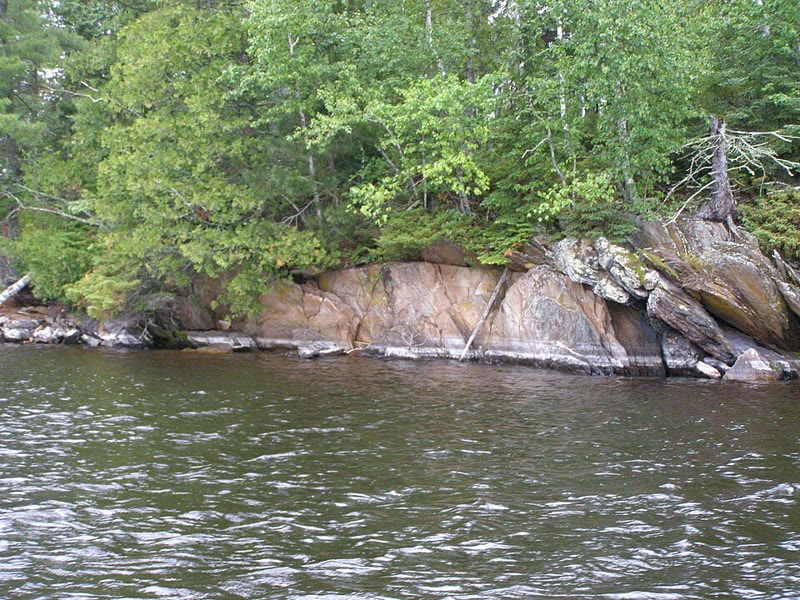
\includegraphics[height=5.0cm]{images/book2/g12-light-canadian-shield.jpg}

{\small Gneises y granitos de 1000 a 3000 millones de años a la orilla de un
lago de Canadá, parte del núcleo antiguo de América del Norte. Fotografía de
Chris Light (CC~BY-SA~4.0).}
\end{omfigure}
% ledger: photo:g12-canadian-shield

¿Por qué perdura la \omterm{def:g12:continental-crust:continental-crust}{corteza continental}, mientras que el fondo oceánico es
siempre joven? La \omterm{def:g11:ocean-ridges:oceanic-lithosphere}{corteza oceánica} es densa: se hunde de nuevo en el manto en
las \omterm{def:g11:subduction-zones:subduction}{zonas de subducción}, y nada de ella sobrevive mucho más de 200 millones de
años. La \omterm{def:g12:continental-crust:continental-crust}{corteza continental} es demasiado ligera para hundirse; puede ser
desgastada por la erosión, estirada o plegada, pero permanece en la
superficie. Las rocas de un continente son un archivo de cuatro mil millones
de años.
% ledger: tulane:no-subduct, tulane:roots, data:b2-seafloor-age

\section{Raíces de montañas}

Cuanto más altas son las montañas, más gruesa es la corteza bajo ellas.

\begin{definition}[Raíz de una cordillera]\label{def:g12:continental-crust:root}
La \emph{raíz}\index{raiz (de una cordillera)@raíz (de una cordillera)} de una
cordillera es la parte de su corteza engrosada que penetra en el manto por
debajo del nivel del \omterm{def:g11:seismic-structure:moho}{Moho} de las llanuras que la rodean.
\end{definition}
% ledger: tulane:roots

El modelo de Airy predice la \omterm{def:g12:continental-crust:root}{raíz}: una cordillera que se eleva $h$ sobre sus
alrededores tiene una \omterm{def:g12:continental-crust:root}{raíz} $r = h\,\rho_c/(\rho_m - \rho_c)$, unas cinco veces
su altura con $\rho_c = \qty{2830}{kg/m^3}$ y $\rho_m =
\qty{3380}{kg/m^3}$ (la \cref{prop:g11:lithosphere-asthenosphere:airy}). Dos
tipos de medidas detectan las raíces. Los sondeos sísmicos encuentran el \omterm{def:g11:seismic-structure:moho}{Moho}
más hondo bajo las cordilleras: de 50 a \qty{70}{km} bajo muchos cinturones
montañosos, unos \qty{70}{km} bajo partes del Tíbet. La gravedad es más débil
sobre las cordilleras de lo que haría pensar su masa visible: la \omterm{def:g12:continental-crust:root}{raíz} ligera,
que ocupa el lugar de un manto más denso, supone un déficit de masa en
profundidad, y las anomalías de la gravedad medidas siguen la topografía y el
espesor de la corteza hallado por la sismología. Los continentes flotan, y sus
montañas flotan más alto que nada.
% ledger: tulane:roots, karplus:tibet-moho, cm95:crust, data:prem

\section{Ejercicios}

\begin{exercise}[$\star$]\label{exo:g12:continental-crust:1}
Copia y completa para la \omterm{def:g12:continental-crust:continental-crust}{corteza continental} y la oceánica: espesor; rocas
principales; contenido en sílice; densidad; edad máxima.
\end{exercise}

\begin{exercise}[$\star$]\label{exo:g12:continental-crust:2}
La \omterm{def:g12:continental-crust:continental-crust}{corteza continental} entera contiene un \qty{60.6}{\percent} de sílice, y su
parte superior un \qty{66.6}{\percent}. Con las clases de sílice de las rocas
ígneas, ¿es cada una \omterm{def:g11:igneous-rocks:felsic-mafic}{máfica}, \omterm{def:g11:igneous-rocks:felsic-mafic}{intermedia} o \omterm{def:g11:igneous-rocks:felsic-mafic}{félsica}? Nombra una \omterm{def:g11:igneous-rocks:volcanic-plutonic}{roca plutónica}
de la misma composición.
\end{exercise}

\begin{exercise}[$\star$]\label{exo:g12:continental-crust:3}
¿Por qué la \omterm{def:g11:ocean-ridges:oceanic-lithosphere}{corteza oceánica} puede hundirse en el manto en una \omterm{def:g11:subduction-zones:subduction}{zona de
subducción}, y la continental no? Responde con densidades.
\end{exercise}

\begin{exercise}[$\star$]\label{exo:g12:continental-crust:4}
(1) ¿Qué es un \omterm{def:g12:continental-crust:craton}{cratón}? (2) ¿Qué edad tienen como mínimo las rocas de un
\omterm{def:g12:continental-crust:craton}{cratón}? (3) ¿Qué tipos de rocas lo forman?
\end{exercise}

\begin{exercise}[$\star$]\label{exo:g12:continental-crust:5}
El fondo oceánico más antiguo tiene unos 190 millones de años; el gneis de
Acasta, 4030 millones de años. ¿Cuántas veces más antiguo es el gneis? ¿Por
qué no hay un fondo oceánico tan antiguo?
\end{exercise}

\begin{exercise}[$\star\star$]\label{exo:g12:continental-crust:6}
La \omterm{def:g12:continental-crust:continental-crust}{corteza continental} cubre \num{210.4}~millones de~\unit{km^2}, de los que
el \qty{30.6}{\percent} está bajo el mar. (1) ¿Qué superficie de \omterm{def:g12:continental-crust:continental-crust}{corteza
continental} está bajo el mar? (2) ¿Qué superficie queda por encima? (3) La
superficie de la Tierra es $4\pi R^2$ con $R = \qty{6371}{km}$. ¿Qué fracción
de la superficie cubre la \omterm{def:g12:continental-crust:continental-crust}{corteza continental}?
\end{exercise}

\begin{exercise}[$\star\star$]\label{exo:g12:continental-crust:7}
Calcula la masa de una columna de corteza de \qty{1}{m^2} de sección, desde
la superficie hasta el \omterm{def:g11:seismic-structure:moho}{Moho}: (1) a través de \qty{41.1}{km} de \omterm{def:g12:continental-crust:continental-crust}{corteza
continental} a \qty{2830}{kg/m^3}; (2) a través de \qty{7.1}{km} de \omterm{def:g11:ocean-ridges:oceanic-lithosphere}{corteza
oceánica} a \qty{3000}{kg/m^3}. (3) ¿Cuántas veces más pesada es la primera?
\end{exercise}

\begin{exercise}[$\star\star$]\label{exo:g12:continental-crust:8}
Una cordillera se eleva \qty{2.5}{km} sobre unas llanuras cuya corteza tiene
\qty{35}{km} de espesor. Con $\rho_c = \qty{2830}{kg/m^3}$ y $\rho_m =
\qty{3380}{kg/m^3}$, calcula su \omterm{def:g12:continental-crust:root}{raíz} y el espesor de su corteza. ¿Está el
resultado dentro del intervalo medido bajo los cinturones montañosos?
\end{exercise}

\begin{exercise}[$\star\star$]\label{exo:g12:continental-crust:9}
A partir del histograma de edades del fondo oceánico: (1) ¿qué fracción del
fondo oceánico tiene menos de 30 millones de años? (2) ¿Qué banda de 10
millones de años contiene más fondo? (3) ¿Por qué baja la fracción hacia las
edades antiguas?
\end{exercise}

\begin{exercise}[$\star\star$]\label{exo:g12:continental-crust:10}
Cartografiada con sus partes sumergidas, la \omterm{def:g12:continental-crust:continental-crust}{corteza continental} tiene una
altura media de unos \qty{120}{m}. Supón que sus partes sumergidas, el
\qty{30.6}{\percent} de su superficie, están por término medio \qty{100}{m}
bajo el nivel del mar. ¿Cuál es la altura media de su parte emergida? ¿Por qué
las estimaciones antiguas, que contaban solo las tierras emergidas, dan una
altura media mucho mayor?
\end{exercise}

\begin{exercise}[$\star\star$]\label{exo:g12:continental-crust:11}
Un sondeo en una isla muy adentrada en un océano alcanza, bajo unos cientos de
metros de lavas, un \omterm{def:g11:ocean-ridges:gabbro}{gabro}; los perfiles sísmicos sitúan el \omterm{def:g11:seismic-structure:moho}{Moho} a \qty{8}{km}
de profundidad. Otro sondeo, bajo una llanura amplia y plana, alcanza gneis a
\qty{2}{km}, y el \omterm{def:g11:seismic-structure:moho}{Moho} está a \qty{38}{km} de profundidad. Usa el método para
decidir qué corteza hay bajo cada uno.
\end{exercise}

\begin{exercise}[$\star\star\star$]\label{exo:g12:continental-crust:12}
¿Qué tan buena es la aproximación de la proposición? (1) Calcula el volumen
exacto de una capa esférica de espesor \qty{41.1}{km} en la superficie de una
esfera de radio \qty{6371}{km}, $\tfrac{4}{3}\pi\bigl(R^3 - (R - H)^3\bigr)$,
y el aproximado, $4\pi R^2 H$. (2) ¿Cuál es la diferencia relativa?
Compárala con $H/R$.
\end{exercise}

\begin{exercise}[$\star\star\star$]\label{exo:g12:continental-crust:13}
Supón que el tercio superior de la \omterm{def:g12:continental-crust:continental-crust}{corteza continental}, en masa, contiene un
\qty{66.6}{\percent} de sílice, y la corteza entera un \qty{60.6}{\percent}.
(1) ¿Cuál es el contenido en sílice de los dos tercios inferiores? (2) ¿A qué
clase de roca ígnea corresponde? (3) ¿Qué dice eso de la \omterm{def:g12:continental-crust:continental-crust}{corteza continental}
profunda?
\end{exercise}

\begin{exercise}[$\star\star\star$]\label{exo:g12:continental-crust:14}
Supón que la nueva \omterm{def:g11:ocean-ridges:oceanic-lithosphere}{corteza oceánica} se forma en las dorsales a razón de unos
\qty{3}{km^2} al año, y que el fondo oceánico cubre unos
\num{300}~millones de~\unit{km^2}. (1) ¿Cuánto tardarían las dorsales en
formar una superficie igual a todo el fondo oceánico? (2) Compáralo con las
edades del fondo oceánico. (3) ¿Qué tiene que ocurrirle al fondo antiguo?
\end{exercise}

\begin{exercise}[$\star\star\star$]\label{exo:g12:continental-crust:15}
Supón que toda la \omterm{def:g12:continental-crust:continental-crust}{corteza continental}, \qty{8.6e9}{km^3}, se hubiera formado
a un ritmo constante desde hace 4000 millones de años. (1) Calcula el ritmo en
kilómetros cúbicos al año. (2) Los circones de las Jack Hills muestran que ya
existía algo de corteza hace 4400 millones de años. ¿Encaja un ritmo
constante con un mundo en el que la mayor parte de la corteza podría haberse
formado pronto, o tarde? ¿Qué podrían decir las rocas más antiguas, y qué no
pueden decir, dado que la corteza antigua puede erosionarse o reciclarse?
\end{exercise}

\section{Problema: ¿cuánto pesa la corteza continental?}

\begin{problem}[{Problema de fin de semana --- la masa de los continentes}]
\label{pb:g12:continental-crust:1}
% ledger: cogley84:continents, cm95:crust, earth:mass, earth:Rmean, earth:density, white92:crust
% values: 4 pi R^2 = 5.1006e8 km2; V = 210.4e6 x 41.1 = 8.647e9 km3; m = 2.447e22 kg; m/M = 0.410 %
La \omterm{def:g12:continental-crust:continental-crust}{corteza continental} cubre \num{210.4}~millones de~\unit{km^2} (incluidas
sus partes sumergidas). Los sondeos sísmicos le dan un espesor medio de
\qty{41.1}{km} y una densidad media de \qty{2830}{kg/m^3}. La Tierra tiene un
radio medio de \qty{6371}{km}, una masa de \qty{5.9722e24}{kg} y una densidad
media de \qty{5513}{kg/m^3}.

\medskip
\noindent\textbf{Parte I --- La superficie.}
\begin{enumerate}
  \item Calcula la superficie de la Tierra, $4\pi R^2$, en
        \unit{km^2}.
  \item ¿Qué fracción de ella cubre la \omterm{def:g12:continental-crust:continental-crust}{corteza continental}?
  \item El \qty{30.6}{\percent} de la \omterm{def:g12:continental-crust:continental-crust}{corteza continental} está bajo el mar.
        ¿Qué superficie es esa?
  \item ¿Qué superficie de la Tierra queda para la \omterm{def:g11:ocean-ridges:oceanic-lithosphere}{corteza oceánica},
        suponiendo que todo el resto es oceánico?
  \item ¿Por qué la \omterm{def:g12:continental-crust:continental-crust}{corteza continental} es más extensa que las tierras emergidas?
\end{enumerate}

\medskip
\noindent\textbf{Parte II --- Espesor y volumen.}
\begin{enumerate}[resume]
  \item ¿Por qué puede calcularse el volumen como superficie por espesor,
        aunque la corteza esté sobre una esfera?
  \item Calcula el volumen de la \omterm{def:g12:continental-crust:continental-crust}{corteza continental} en \unit{km^3}.
  \item Conviértelo a \unit{m^3}.
  \item Otra estimación del espesor medio es \qty{36}{km}. ¿Qué
        volumen da?
  \item ¿En qué porcentaje difieren los dos volúmenes?
\end{enumerate}

\medskip
\noindent\textbf{Parte III --- Densidad y masa.}
\begin{enumerate}[resume]
  \item Calcula la masa de la \omterm{def:g12:continental-crust:continental-crust}{corteza continental} con \qty{41.1}{km}.
  \item Calcula la masa de una columna de \qty{1}{m^2} a través de la
        \omterm{def:g12:continental-crust:continental-crust}{corteza continental}.
  \item Calcula la masa de la \omterm{def:g11:ocean-ridges:oceanic-lithosphere}{corteza oceánica}: superficie de la pregunta~4,
        espesor \qty{7.1}{km}, densidad \qty{3000}{kg/m^3}.
  \item ¿Cuál es más pesada, y cuántas veces? ¿Por qué, si cubre menos
        superficie?
  \item ¿Por qué la \omterm{def:g12:continental-crust:continental-crust}{corteza continental} es menos densa que la oceánica?
\end{enumerate}

\medskip
\noindent\textbf{Parte IV --- Comparada con la Tierra.}
\begin{enumerate}[resume]
  \item Divide la masa de la pregunta~11 por la masa de la Tierra.
  \item Comprueba el resultado con la proposición sobre las capas delgadas.
  \item ¿Qué fracción de la masa de la Tierra es la \omterm{def:g11:ocean-ridges:oceanic-lithosphere}{corteza oceánica}?
  \item La \omterm{def:g12:continental-crust:continental-crust}{corteza continental} contiene las únicas rocas de más de unos 200
        millones de años. ¿Qué fracción de la masa de la Tierra guarda el
        registro de casi toda su historia?
  \item Concluye: ¿qué fracción de la masa de la Tierra es la \omterm{def:g12:continental-crust:continental-crust}{corteza continental}?
\end{enumerate}
\end{problem}
